\documentclass{article}
\usepackage[utf8]{inputenc}
\usepackage{enumitem}

\title{Literature Review: Synthesising emotion-driven images}
\author{Konrad Cybulski}
\date{May 2019}

\usepackage[numbers]{natbib}
\usepackage{graphicx}

\begin{document}
	
\maketitle

\section{Aims and Scope}

The primary focus of the proposed research is to produce an image emotion classifier, and to further leverage it in the process of emotion-driven image synthesis.
The two core themes explored are image generation techniques, and processes for classifying and generating emotional content.
As a result this literature review aims to explore and understand the progression of knowledge in the fields of emotion representation and classification, computational image synthesis, and affective content synthesis.
All of which represent the multiple facets of the proposed body of research with which an investigation into the use of image emotion classifiers for emotion-driven image generation will be explored.

\section{Emotion representation}

The field of emotion classification has surged in recent years given a popularity and rising interest in facial emotion recognition.
Other research has focused on exploring ways in which emotion can be recognised in images, text, and more abstract content.
Underlying these two areas of emotion recognition is the methods for quantitatively representing emotion in both a meaningful, and accurate way.
This section will discuss the evolution of these aspects of emotion classification, in addition to their commonalities, and differences.

The computational recognition of emotion has been explored in countless studies and projects, in both the context of image emotion recognition \citep{machajdik2010affective,zhao2014exploring,kim2018building} and facial emotion classification \citep{mollahosseini2016going}.
However a core component and key difference between a large number of such bodies of research is the method by which emotion is represented.
Two of the most common representations represent a discrete, and continuous approach.
Discrete emotion representations generally involve the categorisation of emotion to a series of labels.
Discrete approaches represent the method used in a large number of papers \citep{machajdik2010affective,ali2017emotional,wangarttalk,mohammad2018wikiart} however the number of emotion labels explored varies greatly.
An example of the size of emotion label subsets used in studies of image emotion classification using such a discrete model are 7 \citep{ali2017emotional}, 8 \citep{machajdik2010affective}, 11 \citep{wangarttalk}, and even 19 \citep{mohammad2018wikiart}.
Due to this lack of consistency in emotion classification targets, such studies often resort to performing similar data gathering and classifier training methods.
Despite the consequences of inconsistency in the emotion labels chosen, due to the simplicity of discrete categorical emotion assignment, data gathering can be performed with ease compared to continuous methods of emotion representation.
In order to create large image datasets of labelled images can be completed with greater ease when the number of such labels is reduced.
However there remains difficulty in labelling images with respect to emotion given the inherent variation in the emotion felt by someone when both viewing an abstract image, or accurately determining the emotion expressed by a facial expression.

The aforementioned difficulty associated with labelling images according to their respective emotional content is accentuated with the introduction of a dimensionally continuous representation of emotion.
While proposed representations vary, the most recognised basis for many continuous models is the circumplex model of emotion \citep{russell1980circumplex}.
The circumplex model of emotion introduced by \citet{russell1980circumplex} asserts that emotion can be measured in terms of two continuous variables: valence, and arousal.
Valence measures the positivity or negativity associated with an emotion; and arousal measures the excitement associated with it.
For example, the discrete emotion label of \textbf{happiness} could be represented in the continuous valence-arousal (VA) space with high-valence, medium-arousal; while the label \textbf{depressed} would translate to low-valence, low-arousal; and \textbf{relaxed} being medium-valence, low-arousal.
While this continuous dimensional model allows for greater continuity in measuring emotions, it is not without fault \citep{larsen1992promises}.
The primary limitations of such a model involve it's likelihood of misinterpretation particularly when considering the labels of each dimension, and any information loss arising from reducing more complex emotions to a two-dimensional space.
One way in which the circumplex model of affect introduced by \citet{russell1980circumplex} has been extended to address its weaknesses is through the introduction of a third-dimension: Dominance, the amount of control associated with an emotion.
Despite its limitations, the circumplex model has been used extensively in the field of psychology \citep{bradley1994measuring,warriner2013norms}, and in computational emotion classification to a limited extent \citep{zhao2016predicting}.

While both models for the representation of emotion have trade-offs, both suffer from issues related to cross-cultural differences in emotion expression and recognition.
Cultures inherently differ with respect to how emotions are both felt and expressed \citep{markus1991culture}; this is becomes increasingly evident when attempting to classify the affective emotion embodied and expressed by more abstract content such as imagery and sound.
The popular image-emotion dataset used for classification known as the International Affective Picture System (IAPS) was shown to have a significantly different valence-arousal assignment for up to 31.74\% of images between Chinese and American young adults \citep{huang2015affective}.
Valence-arousal values assigned to images often vary when considering a group of people.
To address this potential for error in reporting the subjective emotion imparted by content, the self-assessment manikin (SAM) was introduced \citep{lang1980behavioral}.
SAM, as can be seen in Figure \ref{fig:SAM}, was developed to aid in the evaluation of emotion, particularly its translation into the commonly used three dimensions of the circumplex model of affect: valence, arousal, dominance.
It has proved itself as more accurate and effective than other methods of emotion self-assessment while being less complex \citep{bradley1994measuring}.

\begin{figure}[h!]
	\centering
	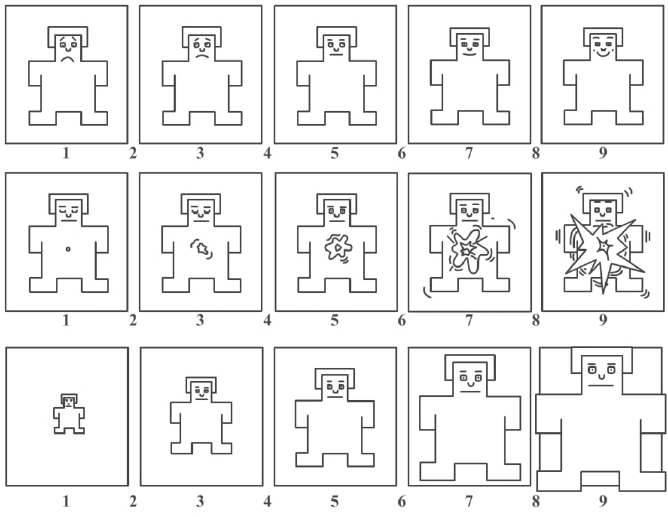
\includegraphics[width=0.75\textwidth]{images/self-assessment-manikin.png}
	\caption{The self-assessment manikin: a guide for reporting individual emotional affect in the three dimensions valence (top), arousal (middle), and dominance (bottom) as introduced by \citet{lang1980behavioral}}
	\label{fig:SAM}
\end{figure}

While both discrete and continuous methods of representing emotion have their respective benefits and trade-offs, the choice to use one over another often depends on the way in which the data gathering process for content emotion classification is performed.
These two representations of emotion can be translated between, since all categorical emotions can be converted to the continuous circumplex model, and the inverse.
However due to the higher complexity nature of the continuous model, even with the use of SAM, dimensional representations are more difficult to gather on a large scale in comparison to categorical emotions.

\section{Emotion classification}

Emotion classification has been researched in depth particularly with respect to two sub-domains: facial emotion recognition, and content emotion classification (image, text, sound).
Facial emotion recognition has been more heavily researched in this field when compared to content emotion classification.

\subsection{Facial emotion recognition}

Humans are known to be more accurate in classifying facial emotion of another when they are culturally similar due to their in-group advantage.
This was also found to be the case with computational facial emotion classifiers when trained more heavily on one culture over another \citep{dailey2010evidence}.



\subsection{Image emotion classification}

\section{Computational image synthesis}

\section{Affective content synthesis}

\section{Conclusion}

\bibliographystyle{apalike}
\bibliography{references}

\end{document}
